\chapter{Problémadefiníció}
A probléma lényege abban keresendő, hogy a korábban kidolgozott általános throughput maximalizáló algoritmus \cite{phd_Hegyhati} valódi ipari környezetben nem minden esetben állja meg a helyét, ugyanis sok esetben a probléma megoldásához használt paraméterek nem determinisztikusak. Változó piaci környezetben ilyen sztochasztikus paraméternek számítanak például a termék iránti kereslet, illetve a piaci ár, amin a terméket értékesíteni lehet. Belátható az is, hogy ezek a paraméterek sokban befolyásolják a maximalizálandó profitot. Vegyünk például egy olyan esetet, amelyben a keresletnél többet termeltünk, ez esetben a keletkező többletet nem tudjuk értékesíteni, ez akár további kiadásokkal is járhat a többlet termék esetleges tárolási költsége miatt. Szakdolgozatom célja a \ref{math_modells} pontban bemutatott, Hegyháti által kidolgozott \cite{phd_Hegyhati} matematikai módszerek segítségével az S-gráf keretrendszer felkészítése a különböző sztochasztikus paraméterek kezelésére, oly módon, hogy az általános throughput maximalizáló algoritmus sértetlen maradjon, a probléma típusától függően kompatibilis használat lehetséges legyen.
\section{A probléma csoportosítása} \label{problem_csop}
A megoldandó problémák a sztochasztikus esetben is az általános throughput maximalizálásnál használt paraméterekkel adottak, pl.: minden terméket a receptje azonosít be, ezen kívül adott a termékek előállítására használható berendezések halmaza, illetve a termelésre rendelkezésre álló időhorizont. Az általános paramétereken kívül azonban sztochasztikus esetben különböző bizonytalanságot kifejező paraméterek is adottak minden termékre, amelyek valószínűségeit különböző scenariokba, forgatókönyvekbe csoportosítjuk. Ezáltal minden forgatókönyvre adott: 
\begin{itemize}
\item{A forgatókönyv valószínűsége}
\item{A termék ára (1 batch ára)}
\item{A termék iránti kereslet}
\item{A túltermelés, az alul termelés költsége}
\end{itemize}
A feladat az, hogy döntést hozzunk a termelt batch-ek darabszámát illetően, miközben egy olyan kivitelezhető ütemtervet biztosítunk, amelyet követve maximális várható profitot érhetünk el.\\
A batch méretekkel kapcsolatos döntések alapján 3 eset különböztethető meg:
\begin{itemize}
\item \textbf{Preventív ütemezés kötött batch mérettel} Ebben az esetben minden termékhez adott egy batch méret, az egyetlen preventív döntés amit hoznunk kell, hogy hány darab batch-et gyártunk az adott termékből.
\item \textbf{Preventív ütemezés változó batch mérettel} Ebben az esetben nem csak a batch darabszám ,de annak a mérete is kiválasztható, de csak preventív módon a bizonytalan események bekövetkezése előtt.
\item \textbf{Két lépcsős ütemezés (two stage)} Ebben az esetben a batch darabszámot előre ki kell választanunk, azonban annak a méretéről a bizonytalan események bekövetkezése után is döntést hozhatunk.
\end{itemize}
Kezdetben feltételezzük, hogy a receptek és a termékek között 1-1 kapcsolat van, azaz egy recept sem eredményez több terméket, illetve egyetlen termék sem állítható elő több fajta recepttel. A \ref{extended_multiproduct} pontban azonban kitérek azokra az esetekre, amelyekben ez a feltételezés nem állja meg a helyét.
\section{A probléma paraméterei} \label{problem_parameters}
A \ref{problem_csop} pontban bevezetett sztochasztikus esetek kezeléséhez az általános throughput maximalizáló algoritmus jelentős része felhasználható változtatások nélkül (vagy csak minimális változtatások árán, lsd. \ref{refactor} pont). Az egyetlen meghatározó különbség az un. "revenue" függvényben figyelhető meg, amely célja, hogy az adott konfigurációra nézve kiszámítsa a várható profitot. A porbléma megoldása során használt paraméterek:
\begin {description}
\item[$P$]  a termékek halmaza
\item[$b_p$]  a legyártott batch-ek darabszáma az adott konfigurációban
\item[$s_p$]  a termék batch mérete (kötött batch méret esetén)
\item[$s_p^{min},s_p^{max}$]  adott termékhez tartozó lehetséges legkisebb, legnagyobb batch méret (válzotó batch méret esetén)
\item[$S$]  a forgatókönyvek halmaza
\item[$prob_s$]  s forgatókönyv valószínűsége $s	\in S$
\item[$dem_{s,p}$]  p termék iránti kereslet az s forgatókönyvben $s	\in S, p	\in P$
\item[$price_{s,p}$]  p termék ára az s forgatókönyvben $s	\in S, p	\in P$
\item[$oc_{s,p}, uc_{s,p}$]  p termék túl-, és alul termelési költsége s forgatókönyvben $s	\in S, p	\in P$
\end {description}
Ezenkívül érdemes bevezetni még a $Profit_{s,p}(x)$ jelölést, amely megadja $x$ mennyiségű $p$ termék bevételét az adott $s$ forgatókönyvben:
\begin{equation*}
Profit_{s,p}(x)= \begin{cases}
            price_{s,p}\cdot x-(dem_{s,p}-x) \cdot uc_{s,p}\qquad \text{ha } x<dem_{s,p} \\
            price_{s,p} \cdot dem_{s,p}-(x-dem_{s,p}) \cdot oc_{s,p}\qquad \text{egyébként}
       \end{cases}
\end{equation*}\\
\begin{figure}
\begin{center}
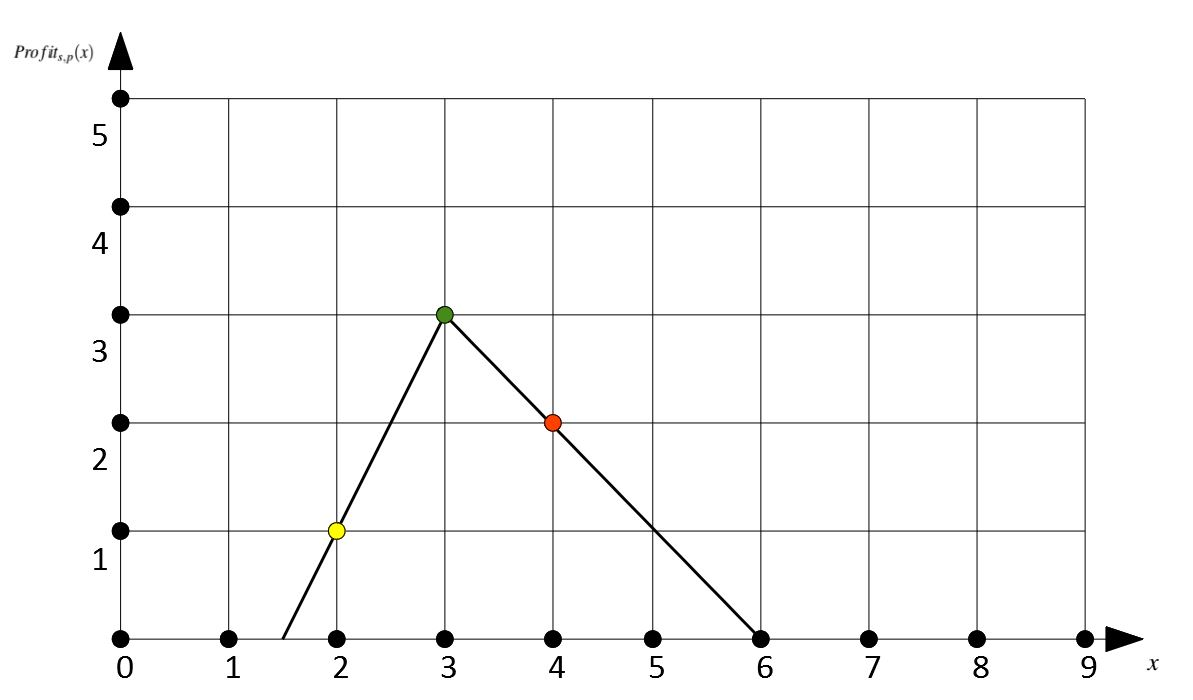
\includegraphics[scale=0.38]{profit_func}
\caption[A profit függvény szemléltetése a következő paraméterekkel:; $s_p=1,\quad dem_{s,p}=3, \quad oc_{s,p}=1, \quad  uc_{s,p}=1$]
    {\tabular[t]{@{}l@{}}A profit függvény szemléltetése a következő paraméterekkel: \\ $s_p=1,\quad dem_{s,p}=3, \quad oc_{s,p}=1, \quad  uc_{s,p}=1$\endtabular}
\label{profit_func}
\end{center}
\end{figure}
Jól látszik, hogy adott termék bevétele akkor lesz maximális, ha a kereslettel egyező darabszámot gyártunk az adott termékből (zöld pont a \ref{profit_func} ábrán), ha ennél kevesebbet gyártunk a termékből, akkor a kereslet kielégítéséből eredő profit is elmarad, illetve további többlet költség kerül levonásra a profit összegéből az esetleges alul termelési plusz költségek miatt (pl. sárga pont a \ref{profit_func} ábrán), abban az esetben pedig, ha a keresletet meghaladó mennyiséget gyártunk adott termékből, a kereslet kielégítődik ugyan, és bevételünk maximális lenne az adott piaci keresletet figyelembe véve, azonban a túltermelés következtében létrejött többlet tárolási költségét le kell vonjuk a profit értékéből (pl. piros pont a \ref{profit_func} ábrán) \footnote{Előfordulhat olyan eset, amelyben az alul-, és túltermelési költségekkel nem kell számolni, ebben az esetben a kereslet értékének eléréséig a profit a termelt mennyiséggel arányosan lineárisan növekedni fog, majd onnantól kezdve konstans módon beáll a maximális értékre, ugyanis a felesleg értékesítése nem lehetséges, ha arra nincs kereslet, viszont annak tárolás nem okoz plusz költséget.}. Arra kell törekedni tehát, hogy a lehetőségeket mérlegelve minden termékből annyit gyártsunk, hogy az az adott forgatókönyvben szereplő keresletet kielégítse, vagy azt a legkedvezőbb módon megközelítse valamelyik irányból, ügyelve az alul-, és túltermelési költségekre. Extrém esetekben előállhat olyan helyzet is, hogy a rendelkezésre álló determinisztikus paraméterek (pl. gépek száma), az aktuális időhorizont, illetve a sztochasztikus paraméterek aktuális értéke miatt a profit függvény $x$-ben felvett értéke negatív szám lesz, ez esetben inkább a veszteségek minimalizálásáról beszélhetünk, mintsem profit maximalizálásról, azonban könnyen belátható, hogy a definiált matematikai modellekben amelyeket használunk a profit kiszámítására, ez semmiféle változást nem eredményez, csupán arra kell figyelni, hogy az implementáció során felkészüljünk a negatív számok a programnyelvben történő kezelésére.